%Old Version from Greg. Greg, this slide is changed substantially, please take a look.
%% begin module algebraic-functions
%\begin{frame}
%\frametitle{Algebraic Functions}
%\begin{definition}[Algebraic Function]
%An algebraic function is a function that can be constructed using algebraic operations (such as addition, subtraction, multiplication, division, and taking roots) starting from polynomials.
%\end{definition}
%\uncover<2->{
%Algebraic functions can look pretty funny.
%\begin{tabular}{ccc}
%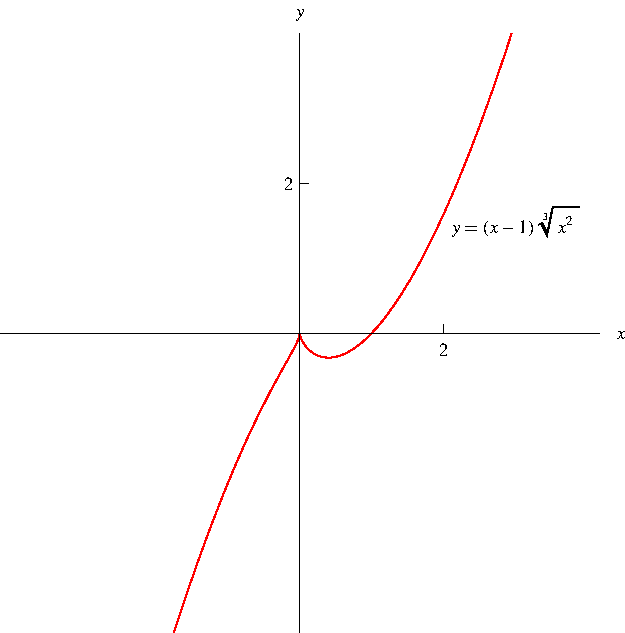
\includegraphics[height=3.8cm]{precalculus/pictures/01-02-algebraic1.pdf}&%
%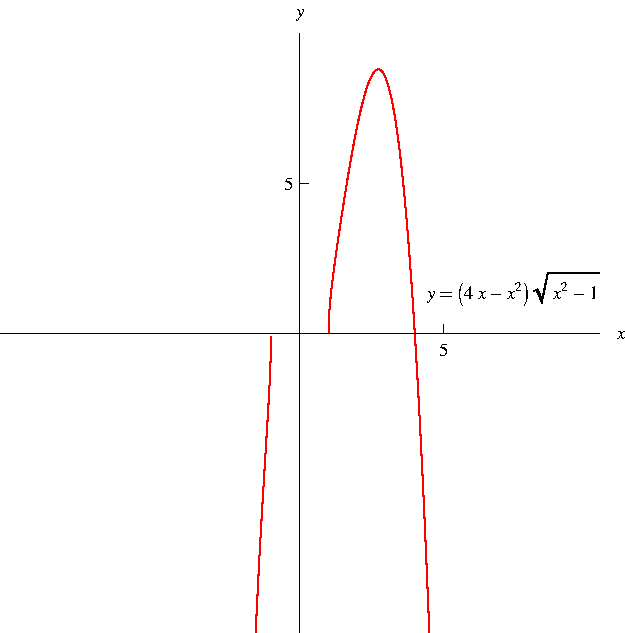
\includegraphics[height=3.8cm]{precalculus/pictures/01-02-algebraic2.pdf}&%
%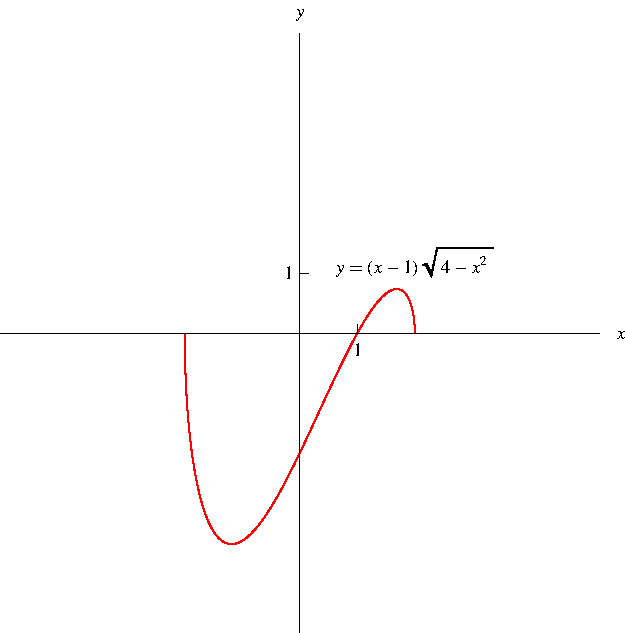
\includegraphics[height=3.8cm]{precalculus/pictures/01-02-algebraic3.pdf}%
%\end{tabular}
%}
%\end{frame}
%% end module algebraic-functions


% begin module algebraic-functions
\begin{frame}
\frametitle{Algebraic Functions}
\begin{definition}[Algebraic Function]
A function in $x$ that can be constructed using $x$, constants, and finitely many of the operations $+, -, *, /,$ and $\sqrt[n]{~}$ is an algebraic function.

\uncover<2->{{\footnotesize Outside of Calculus I: function $f(x)$ = algebraic if it satisfies a polynomial equation with polynomial coefficients, i.e., $a_0(x) +a_1(x)f(x)+\dots +a_n(x) \left(f(x)\right)^n=0$ for some polynomials  $a_i(x)$.}}
\end{definition}
\uncover<3->{
Examples.

\begin{tabular}{ccc}
\psset{xunit=0.3cm, yunit=0.3cm}
\begin{pspicture}(-5, -5)(5,5)
\tiny\psframe*[linecolor=white](-5,-5)(5,5)
\psaxes[ticks=none, labels=none]{<->}(0,0)(-4.5,-4.5)(4.5,4.5)\tiny
%Function formula: - ((- (x))^{5/3})- ((- (x))^{2/3})
\psplot[linecolor=red, plotpoints=1000]{-2}{-0.001}{x -1 mul 0.666667 exp -1 mul x -1 mul 1.66667 exp -1 mul add } %Function formula: (x)^{5/3}- ((x)^{2/3})
\rput[t](1,-5){$y=(x-1)\sqrt[3]{x^2}$}
\psplot[linecolor=red, plotpoints=1000]{0.001}{3}{x 0.666667 exp -1 mul x 1.66667 exp add }
\fcLabels{4.5}{4.5}
\end{pspicture}
%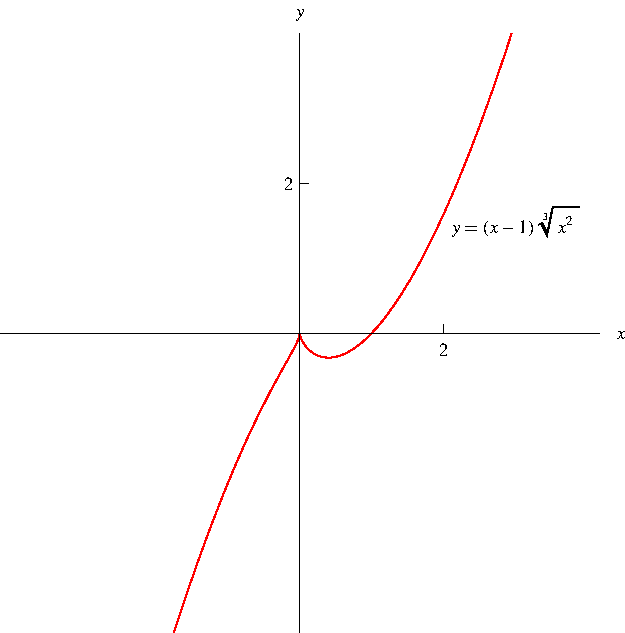
\includegraphics[height=3.8cm]{precalculus/pictures/01-02-algebraic1.pdf}
&%
\psset{xunit=0.3cm, yunit=0.3cm}
\begin{pspicture}(-5, -5)(5,5)
\tiny\psframe*[linecolor=white](-5,-5)(5,5)
\psaxes[ticks=none, labels=none]{<->}(0,0)(-4.5,-4.5)(4.5,4.5)\tiny
\psplot[linecolor=red, plotpoints=1000]{1}{5}{-1 x 2 exp add 0.5 exp x 2 exp mul -0.2 mul -1 x 2 exp add 0.5 exp x mul 0.8 mul add } %Function formula: 4/5 ((x) (((x)^{2}-1)^{1/2}))-1/5 (((x)^{2}) (((x)^{2}-1)^{1/2}))
\rput[t](1,-5){$y=\frac15(4x-x^2)\sqrt{x^2-1}$}
\psplot[linecolor=red, plotpoints=1000]{-2}{-1}{-1 x 2 exp add 0.5 exp x 2 exp mul -0.2 mul -1 x 2 exp add 0.5 exp x mul 0.8 mul add }
\fcLabels{4.5}{4.5}
\end{pspicture}
%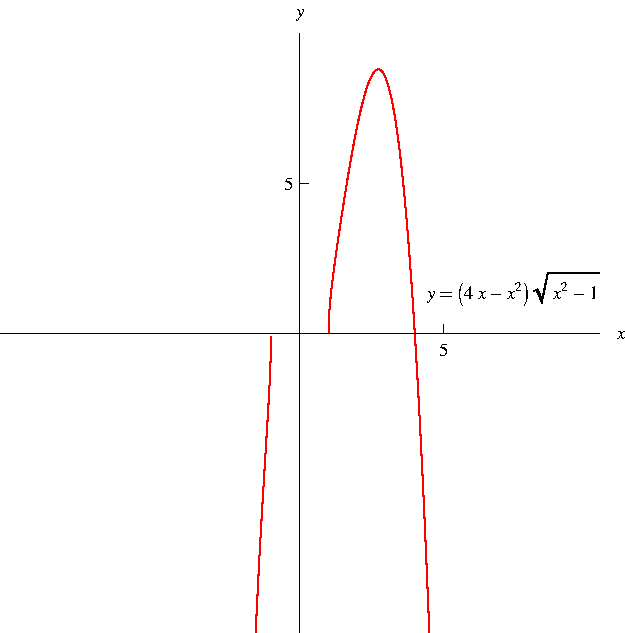
\includegraphics[height=3.8cm]{precalculus/pictures/01-02-algebraic2.pdf}
&%
\psset{xunit=0.3cm, yunit=0.3cm}
\begin{pspicture}(-5, -5)(5,5)
\tiny\psframe*[linecolor=white](-5,-5)(5,5)
\psaxes[ticks=none, labels=none]{<->}(0,0)(-4.5,-4.5)(4.5,4.5)\tiny
%Function formula: - ((4- ((x)^{2}))^{1/2})+(x) ((4- ((x)^{2}))^{1/2})
\rput[t](1,-5){$y=(x-1)\sqrt{4-x^2}$}
\psplot[linecolor=red, plotpoints=1000]{-2}{2}{x 2 exp -1 mul 4 add 0.5 exp x mul x 2 exp -1 mul 4 add 0.5 exp -1 mul add }
\fcLabels{4.5}{4.5}
\end{pspicture}
%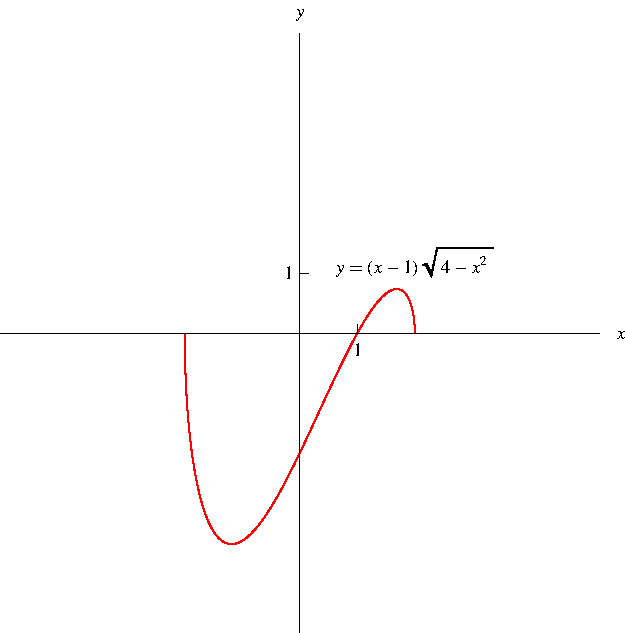
\includegraphics[height=3.8cm]{precalculus/pictures/01-02-algebraic3.pdf}
%
\end{tabular}
}
\end{frame}
% end module algebraic-functions
